\documentclass[10pt,a4paper]{article}

\usepackage[margin=2.1cm]{geometry}
\usepackage{graphicx}
\usepackage{booktabs}
\usepackage{caption}
\usepackage{microtype}
\usepackage{amsmath}
\usepackage{amssymb}
\usepackage[table]{xcolor}
\usepackage[colorlinks=true,linkcolor=black,urlcolor=blue!60!black,citecolor=black]{hyperref}

\captionsetup{font=small,labelfont=bf,width=0.95\textwidth}
\renewcommand{\topfraction}{0.92}
\renewcommand{\bottomfraction}{0.75}
\renewcommand{\textfraction}{0.07}
\renewcommand{\floatpagefraction}{0.80}
\setlength{\parskip}{0.35em}
\setlength{\parindent}{0pt}

\newcommand{\net}[1]{\textsc{#1}}

\title{\vspace{-1.4cm}\textbf{Opinion Network Formation:\\Three Readings of One Class Survey}}
\author{Team: \textbf{A Shortest Path to an A Grade}\\[0.25em]
Vishal \quad$\cdot$\quad Harith \quad$\cdot$\quad Navneet}
\date{Dynamical Processes in Complex Networks --- Assignment 1\\[0.2em]
20 September 2026}

\begin{document}
\maketitle
\vspace{-0.9em}

\begin{center}
\fbox{\begin{minipage}{0.93\textwidth}
\small
\textbf{Code:} \url{https://github.com/Fresh-butter/DPCN_Assignment_1} \\
\textit{Repository layout:} \texttt{common/} (shared data contract and palette),
\texttt{member\_a\_agreement\_net/}, \texttt{member\_b\_statement\_net/},
\texttt{member\_c\_bipartite\_net/}, \texttt{cross\_analysis/}, \texttt{report/}.
Each member's notebook runs standalone and regenerates every figure and table it cites.
\end{minipage}}
\end{center}

\vspace{0.4em}

\section*{The problem this survey poses}

Eighty percent of this class agrees with almost everything. Of the 5158 answers actually
given across 60 statements, 4127 are ``Agree'' or ``Strongly Agree'', and the per-item
means cluster between 3.5 and 4.5 on a five-point scale. Taken at face value, the survey
describes a cohort with essentially one opinion, and the naive network confirms it:
cosine similarity between raw response vectors sits near 0.96 for every pair of students,
which yields a near-complete graph carrying no information at all.

That ceiling is the central analytical problem of this assignment, and it shapes
everything that follows. The interesting quantity is not what a student answered but how
far that answer sat from what everyone else said. Once responses are centred per item,
structure appears --- and it turns out to be considerable, highly non-random, and
organised along lines the survey's own designers did not anticipate.

We built three networks from the one dataset. They differ not in preprocessing but in
what they treat as a node and what they treat as a relationship, and consequently they
answer different questions. The most useful results in this report come from comparing
them: where two independent constructions agree, the agreement is evidence; where they
disagree, the disagreement turns out to be the finding.

\section{Dataset documentation}

The raw file is $96 \times 61$: one respondent identifier and 60 Likert statements,
arranged in four topical blocks of fifteen --- \textbf{T}echnology, \textbf{E}ducation,
\textbf{S}ociety/Ethics, and en\textbf{V}ironment. All cleaning is implemented once, in
\texttt{common/contract.py}, and imported by all three members; no member re-cleans the
data independently.

\begin{table}[h]
\centering
\small
\begin{tabular}{@{}llp{8.6cm}@{}}
\toprule
\textbf{Step} & \textbf{Result} & \textbf{Rationale} \\
\midrule
Encode Likert 1--5 & numeric & Strongly Disagree $=1$ \dots\ Strongly Agree $=5$. \\
``No Comments''/blank $\to$ NaN & --- & Never encoded as 3. Treating a non-answer as
``Neutral'' fabricates data at the exact centre of the scale and biases every
correlation toward zero. \\
Drop rows with $>30$ of 60 missing & $96 \to 87$ & The cutoff is read off the data, not
chosen (see below). \\
Respondents $\times$ items matrix & $87 \times 60$ & 62 missing cells remain. \\
Per-item $z$-score, computed on all 87 & --- & Mandatory, not stylistic; see below. \\
\bottomrule
\end{tabular}
\end{table}

\textbf{Why 30.} The distribution of missing answers per row has a clean natural break.
Sixty-eight rows have no missing answers and a further seventeen have between one and
four; one row each has 10 and 15; the count then jumps directly to 45 (four rows) and 60
(five rows). Nothing whatsoever falls between 15 and 45, so any threshold inside that gap
retains exactly the same 87 respondents. The nine rows dropped are abandoned responses
rather than partial ones, which is a materially different thing to discard.

\textbf{Why $z$-score.} This is the step that makes the rest of the analysis possible.
Raw pairwise correlation between students averages $0.267$; after centring each item on
its own mean, pairwise-complete cosine similarity averages $-0.010$ and spreads across
$[-0.638, +0.758]$. The ceiling is removed and genuine variation becomes visible.
Standardisation is performed over the full 87 respondents so that all three members'
$z$-values share one reference frame.

\textbf{What we deliberately did not standardise.} Handling of the 62 remaining missing
cells is a modelling choice rather than a cleaning one, so each construction treats it
differently: pairwise-complete cosine requiring at least 20 shared items (A),
pairwise-complete Pearson with \texttt{min\_periods=10} (B), and simply no edge for a
missing cell (C). Each member additionally reports a mean-imputed variant as a
sensitivity check; the differences are negligible (for B, mean $|\Delta r| = 0.0033$).

Two items, E02 and T10, were flagged as possibly reverse-worded. We flagged them rather
than flipping them, on the grounds that a signed network should be allowed to discover
reverse-coding as negative edges rather than have it silently corrected away beforehand.
E02 does behave as a genuine minority-opinion item; T10 does not, sitting comfortably
inside the majority cluster.

Because all three constructions import the same loader, the three pipelines produce
bit-identical $87 \times 60$ matrices. This is what licenses the cross-network
comparisons in Section 4: A and C describe the same 87 students, B and C the same 60
statements, so every comparison is one population measured two ways rather than two
populations compared.

\section{Pipeline}

\begin{table}[h]
\centering
\footnotesize
\setlength{\tabcolsep}{4pt}
\begin{tabular}{@{}lllrl@{}}
\toprule
& \textbf{Nodes} & \textbf{Edge rule} & \textbf{Edges} & \textbf{Question it answers} \\
\midrule
\textbf{A} Agreement & 87 students & cosine of $z$-vectors $>0.15$ & 822 & Who thinks alike? \\
\textbf{B} Signed statement & 60 statements & Pearson $r$, permutation, FDR & 402 & Which opinions move together or clash? \\
\textbf{C} Bipartite deviation & 87 students, 60 items & student--item edge, $|z|>1$ & 1200 & Who breaks consensus, on what? \\
\bottomrule
\end{tabular}
\setlength{\tabcolsep}{6pt}
\end{table}

\textbf{A --- agreement network.} Students are joined when their $z$-scored response
vectors are sufficiently aligned. A threshold of $0.15$ gives 822 edges, mean degree
18.9, and a single connected component. The choice is not knife-edge: sweeping the
threshold, the giant component holds every node up to $0.225$ and only falls below half
the class past $0.325$. A mutual-$k$NN rule ($k=8$) was built as an alternative and
retained for the dynamics in Section 3.4.

\textbf{B --- signed statement network.} Statements are joined by the Pearson correlation
of their response profiles across students, with the sign retained so that opposition is
representable. Significance is assessed against a permutation null in which each item is
independently shuffled, with Benjamini--Hochberg FDR control at $q=0.05$; 402 of 1770
candidate pairs survive, the smallest retained $|r|$ being $0.274$. An earlier attempt
used a family-wise max-statistic threshold, which demanded $|r| > 0.50$ and eliminated
every negative edge --- defeating the purpose of building a signed network at all. The
per-edge FDR rule keeps 391 positive and 11 negative edges.

\textbf{C --- bipartite deviation network.} Rather than removing the ceiling effect and
studying what remains, this construction makes the residual itself the object of study. A
student is joined to a statement when they answered it more than one standard deviation
from the class mean, weighted by $|z|$. At a cutoff of $1.0$ this gives 1200 edges, with
every student and every statement participating.

Every threshold above is arbitrary in the sense that a defensible neighbouring value
exists, so each was swept. The honest summary is that coarse structure is robust while
fine detail is not: A's threshold and $k$NN rules share only 25.2\% of their edges by
Jaccard overlap yet return the same two-community partition, and C's cutoff range
$0.75$--$1.5$ swings the edge count from 2856 to 442 without changing any conclusion
below.

All results use \texttt{SEED = 42}. We additionally require that two consecutive full
re-runs produce byte-identical CSVs, which a fixed seed alone does not guarantee: three
separate code paths iterated over Python sets, letting per-process hash randomisation
reach the results. All now iterate in sorted order.

\begin{figure}[h]
\centering
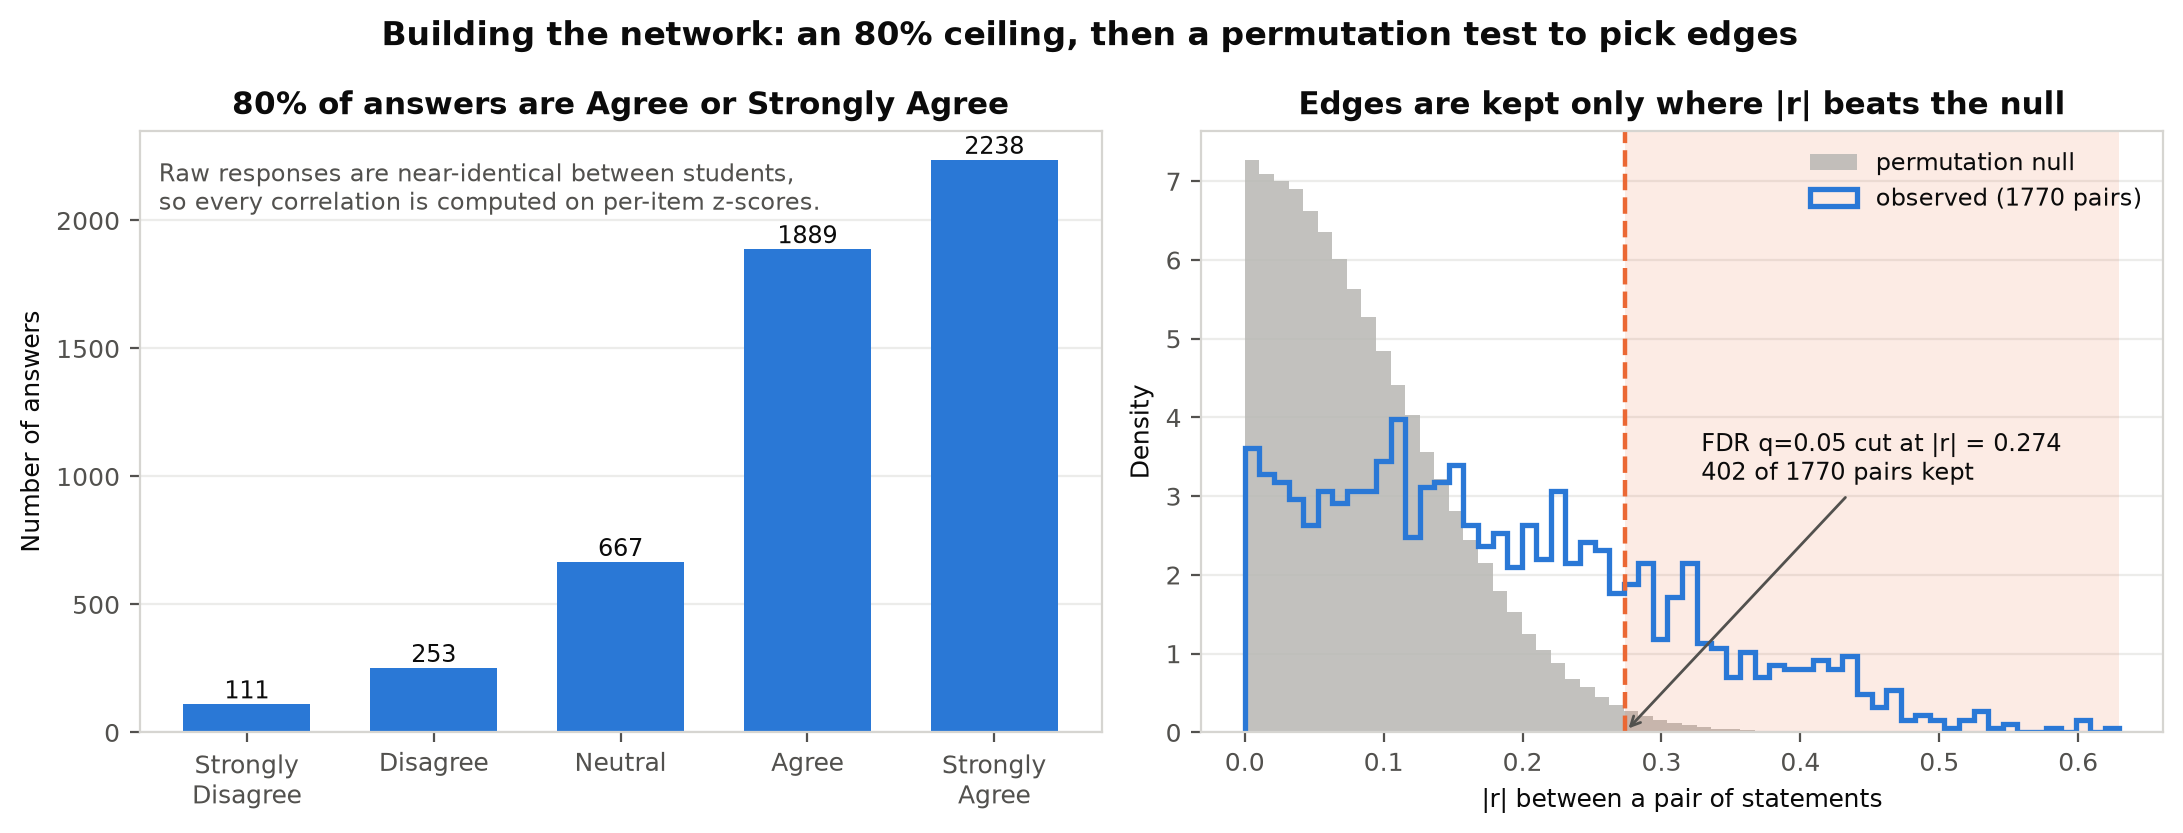
\includegraphics[width=0.92\textwidth]{../member_b_statement_net/figures/fig01_construction.png}
\caption{The problem and one response to it. \textit{Left:} the response distribution ---
80\% of answers given are Agree or Strongly Agree, which is why every construction in this
report operates on $z$-scores rather than raw responses. \textit{Right:} the observed
distribution of $|r|$ across all 1770 statement pairs sits clearly to the right of a
permutation null, and the FDR cut at $|r| = 0.274$ retains exactly the part that
separates.}
\end{figure}

\section{Analysis and visualisations}

\subsection{The class divides into two blocs, and the division is one of intensity}

Louvain on the agreement network returns two substantial communities of 48 and 35
students (plus two negligible pairs) at modularity $Q = 0.432$. Modularity alone proves
nothing, since Louvain returns some partition for any graph whatsoever; the relevant
comparison is against a degree-preserving configuration model, which scores
$0.178 \pm 0.007$ over 30 rewirings. The observed value sits \textbf{35.5 standard
deviations above chance}. The partition is also strongly assortative: 746 of 822 edges
(90.8\%) fall within a community, and within-community edges carry more weight than
between-community ones (0.286 against 0.212).

The same network is far more transitive than chance allows. Average local clustering is
$0.505$ against an Erd\H{o}s--R\'enyi null of $0.220 \pm 0.009$, some 32 standard
deviations above --- if a student agrees with two others, those two very probably agree
with each other. Interestingly, average shortest path length ($2.054$) is slightly
\textit{longer} than the null's ($1.792$): this network is locally cliquey rather than
small-world, clustered but not rich in shortcuts.

\begin{figure}[h]
\centering
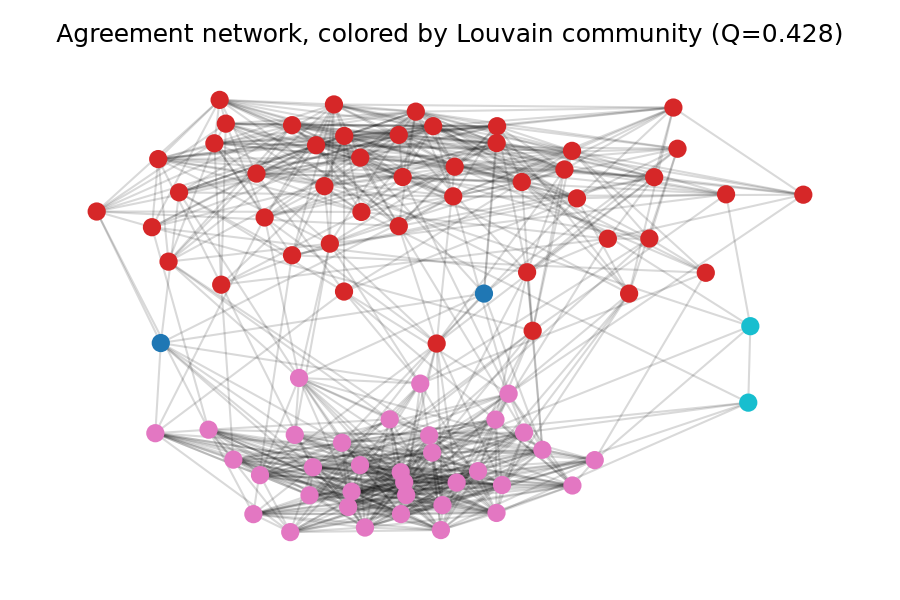
\includegraphics[width=0.52\textwidth]{../member_a_agreement_net/figures/fig04_network_communities.png}
\caption{The agreement network over 87 students, coloured by Louvain community. The two
substantial blocs are visually obvious and statistically far from random
($Q = 0.432$ against a configuration null of $0.178 \pm 0.007$).}
\end{figure}

Profiling what the two blocs actually believe produces the more interesting result. They
are not opposed camps. Both rank the same statements highest; they differ in how hard
they agree. One bloc (35 students) has overall mean $z$ of $+0.371$, the other (48
students) $-0.283$. The division is one of conviction rather than of position --- a
fervent bloc and a temperate one, not a pro- and an anti- faction.

Where that intensity gap lives is sharply concentrated. Of the twenty statements that
best separate the blocs, eleven are Environment and seven are Society/Ethics; only one
each is Technology or Education. Mean absolute $z$-gap per item by block runs
V $0.986$, S $0.835$, E $0.536$, T $0.434$.

\begin{figure}[h]
\centering
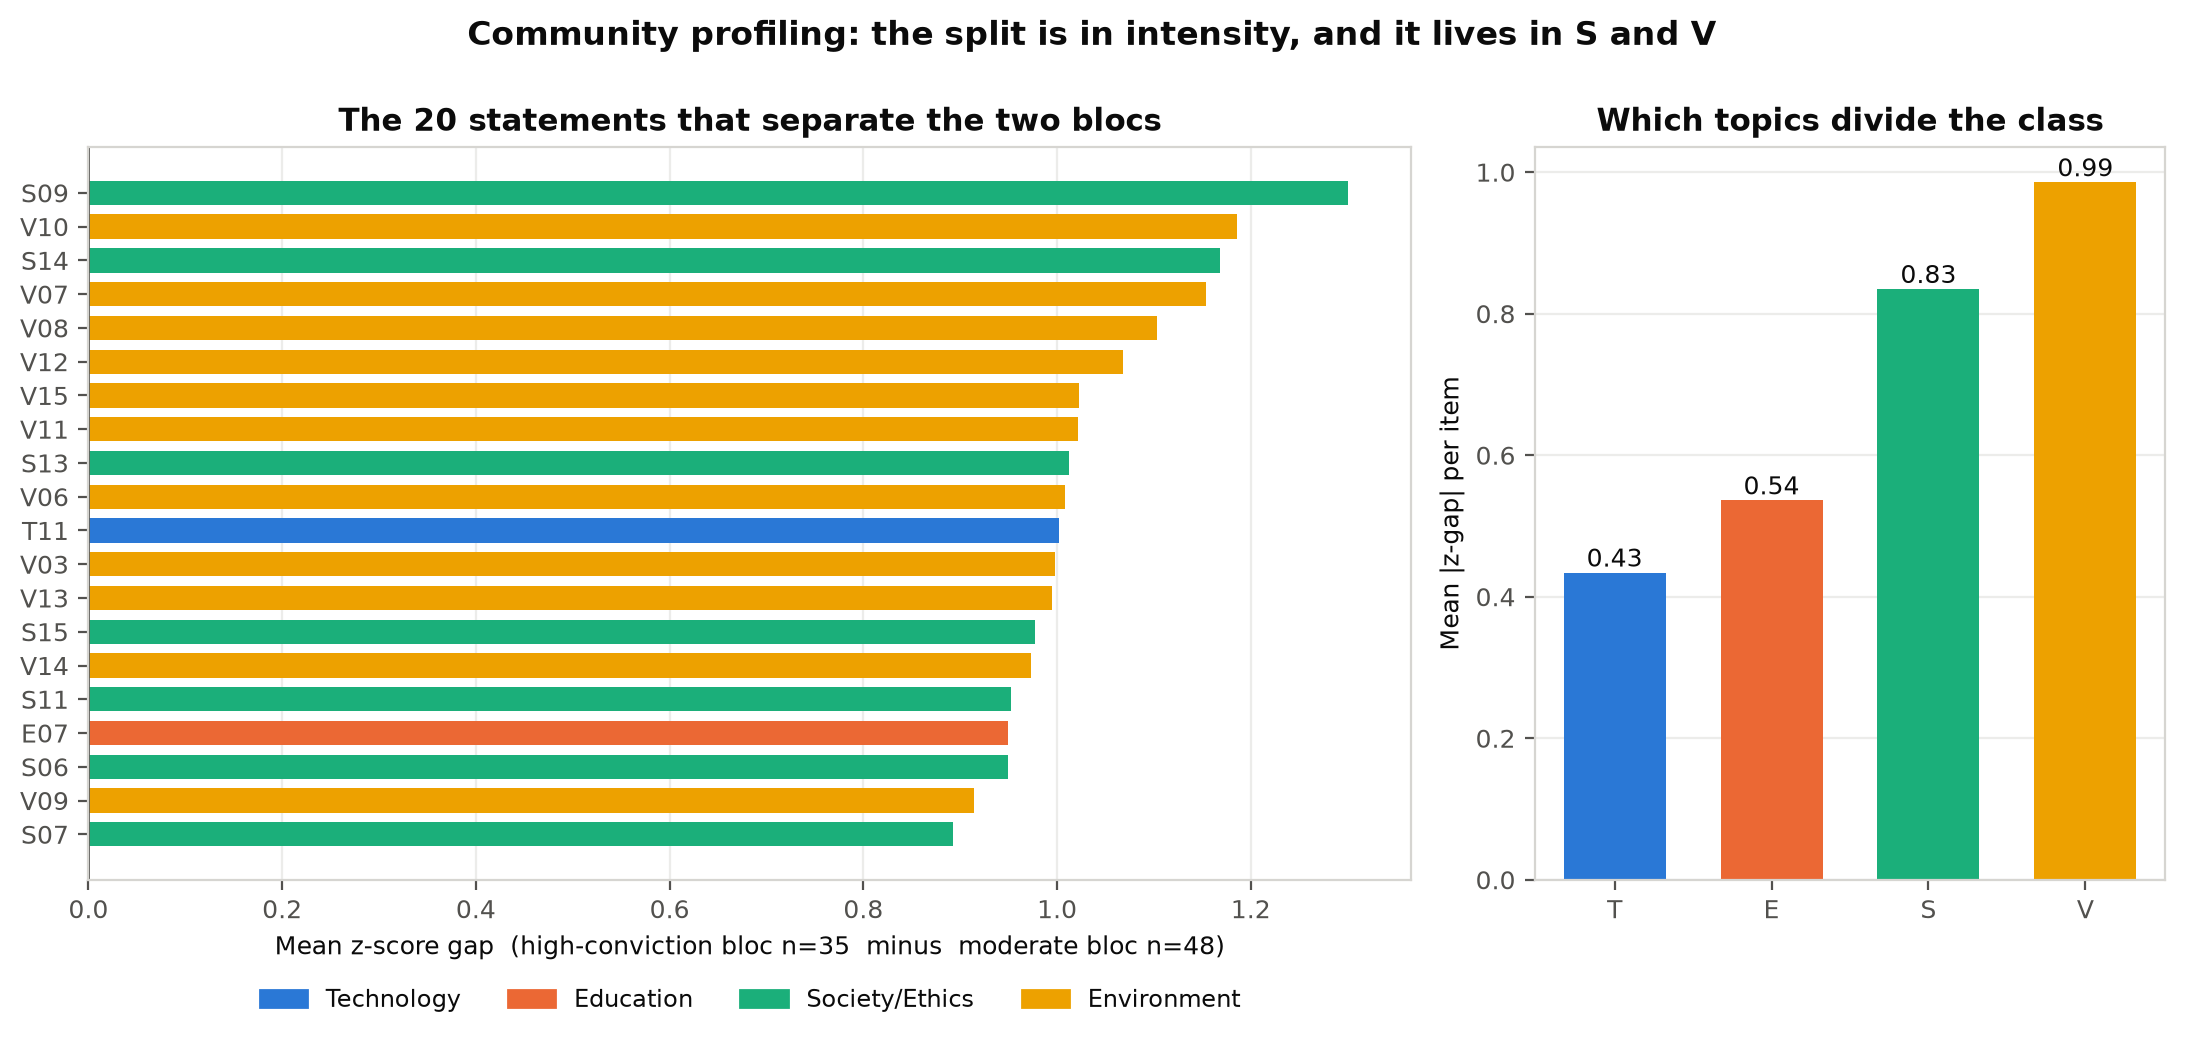
\includegraphics[width=0.92\textwidth]{../member_a_agreement_net/figures/fig07_community_profile.png}
\caption{What separates the two blocs. \textit{Left:} the twenty most discriminating
statements, of which eighteen are Environment or Society/Ethics. \textit{Right:} the same
result aggregated by block. The class divides over how strongly to hold environmental and
social positions, not over technology or education.}
\end{figure}

\subsection{Disagreement is rare, but it is not scattered}

The signed statement network is overwhelmingly positive: 391 of 402 edges. The eleven
negative edges are the interesting ones, and they are not noise distributed at random.
Eight of the eleven touch a single statement, E03 (``Class attendance should be compulsory
for all courses''), which anti-correlates with a coherent cluster of
progressive-education and innovation items (E04, E07, E10, E11, E12, T06, S06). What
looks at first like scattered dissent is in fact one axis: traditionalist versus
progressive pedagogy.

The network is also almost perfectly balanced in the structural sense. Of 1298 closed
triads, \textbf{zero} are frustrated --- every triangle that exists can be consistently
signed. The frustration index, the minimum number of sign flips needed for a clean
two-faction split, is 2 of 402 edges; a null that reshuffles which edges carry the eleven
negative signs while holding topology fixed yields $10.98 \pm 0.16$, placing the observed
value 56 standard deviations \textit{below} chance. (That the triangle census is perfect
while the frustration index is 2 means those two awkward edges sit on a longer signed
cycle that a triangle-only check cannot see.) Whatever this class believes, it believes
it coherently: there are essentially no cases of holding two positions that contradict
each other.

One further result cuts against the survey's own design. Louvain on the positive backbone
finds eight communities whose agreement with the T/E/S/V blocks is weak (NMI $= 0.277$).
The class does not organise its opinions along the topic boundaries the survey assumes.
The clearest symptom is that T08 (AI-assisted diagnosis) and T09 (autonomous vehicles)
survive the FDR cut with \textit{no edges at all} --- two Technology statements that
correlate with nothing else in the survey, including the rest of Technology.

\begin{figure}[h]
\centering
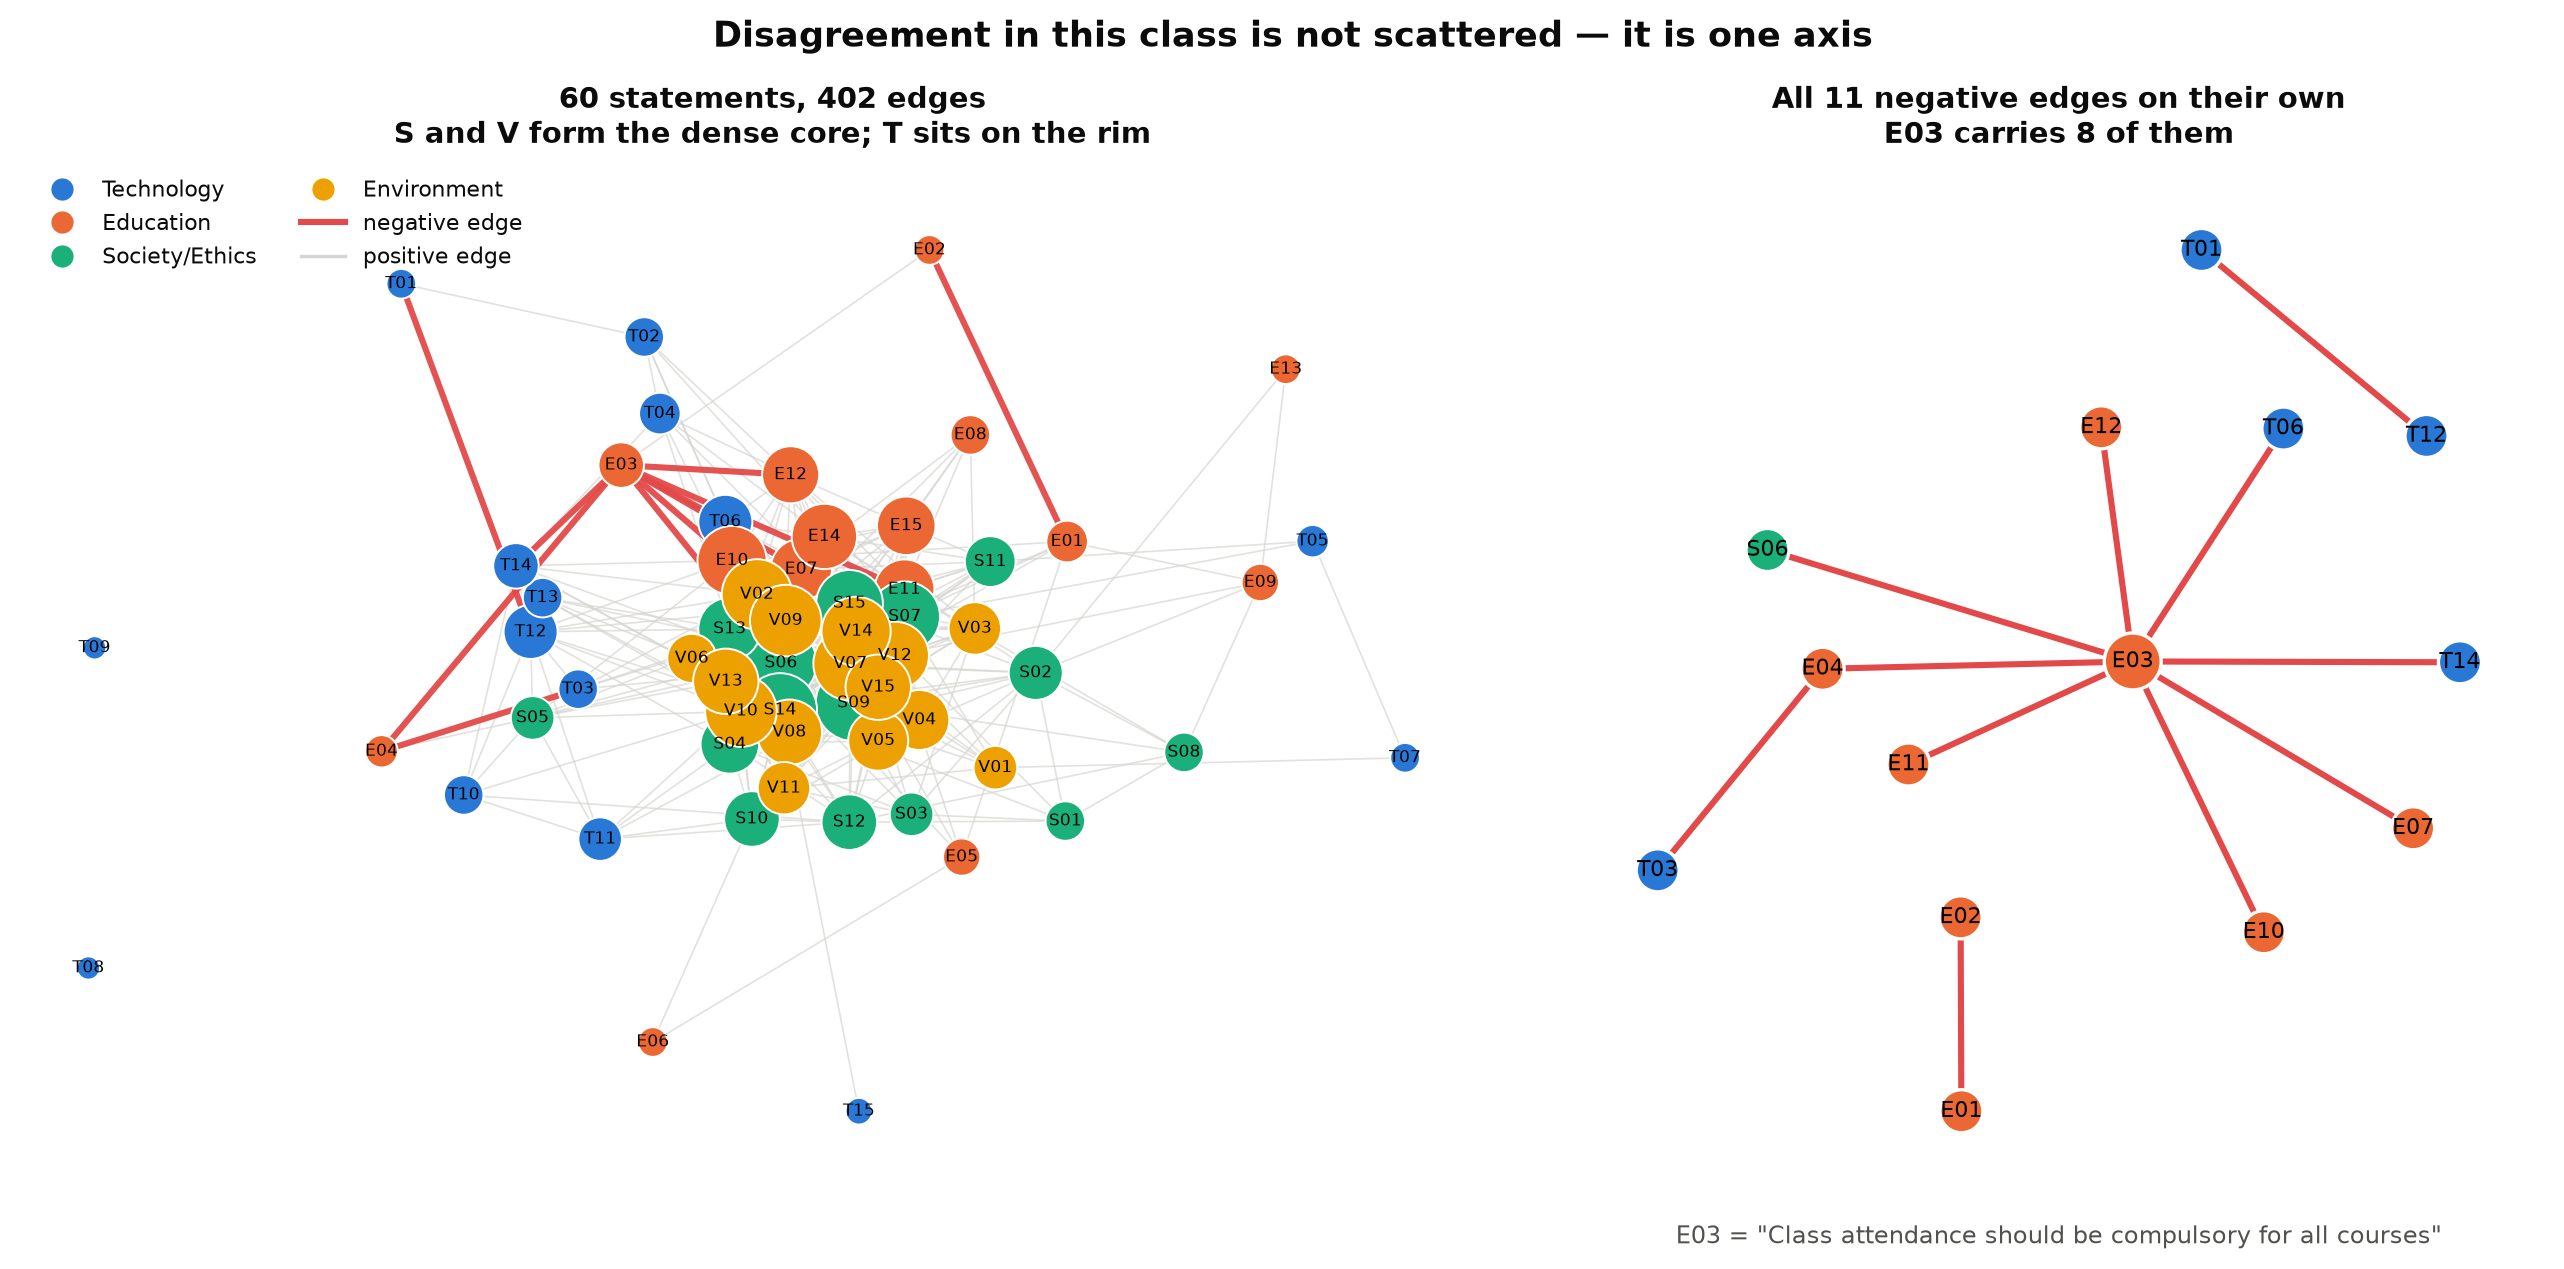
\includegraphics[width=0.95\textwidth]{../member_b_statement_net/figures/fig02_signed_network.png}
\caption{The signed statement network. \textit{Left:} Society and Environment statements
form a dense core while Technology sits on the rim, with T08 and T09 fully isolated.
\textit{Right:} all eleven negative edges drawn alone; E03 carries eight of them.}
\end{figure}

\subsection{Consensus has structure; dissent does not}

The bipartite construction asks the opposite question --- not who agrees, but who breaks
ranks and on what. The most deviated-on statement is T13 (cybersecurity investment), on
which 60 of 87 students answered more than one standard deviation from the mean. Notably,
the lowest-mean items are \textit{not} the highest-deviation items: E03 and E02, which sit
at the centre of B's disagreement structure, rank eleventh and below here. A low mean
means the class agrees a statement is false; a high deviation degree means the class
cannot settle. These are different things.

Projecting the bipartite graph onto its 87 students --- joining two students when they
deviate on the same issues --- produces the result that most surprised us. Louvain returns
two communities at $Q = 0.0368$, which is low; but low is not the same as absent, so we
compared it to a degree-preserving null exactly as for network A. The null scores
$0.0567 \pm 0.0032$. The co-dissent network is therefore not weakly clustered but
\textbf{6.1 standard deviations \textit{less} clustered than chance} --- a random graph
with the identical degree sequence partitions better than the real one.

Set against A's $+35.5$ on the same 87 students, the contrast is the central finding of
this report. When students are linked by what they agree about, they fall into two sharp
camps. When the very same students are linked by what they dissent about, they fall into
nothing at all. There is no contrarian clique; breaking with the class on one issue
predicts nothing about what else you break with.

Sorting the incidence matrix by degree does produce a visibly nested, triangular pattern,
and NODF $= 41.8$ invites the reading that dissent is hierarchical --- that students work
down a shared ordering of contentiousness. That reading does not survive a null either.
NODF rises mechanically with degree heterogeneity, and degrees here span 3 to 35
deviations per student. Against a curveball null fixing both degree sequences, the null
NODF is $41.00 \pm 0.26$: the observed value clears it by $+0.79$ points on a 0--100
scale ($z = +3.08$). Formally above chance, substantively nothing. The apparent hierarchy
is a restatement of the degree sequence.

\begin{figure}[h]
\centering
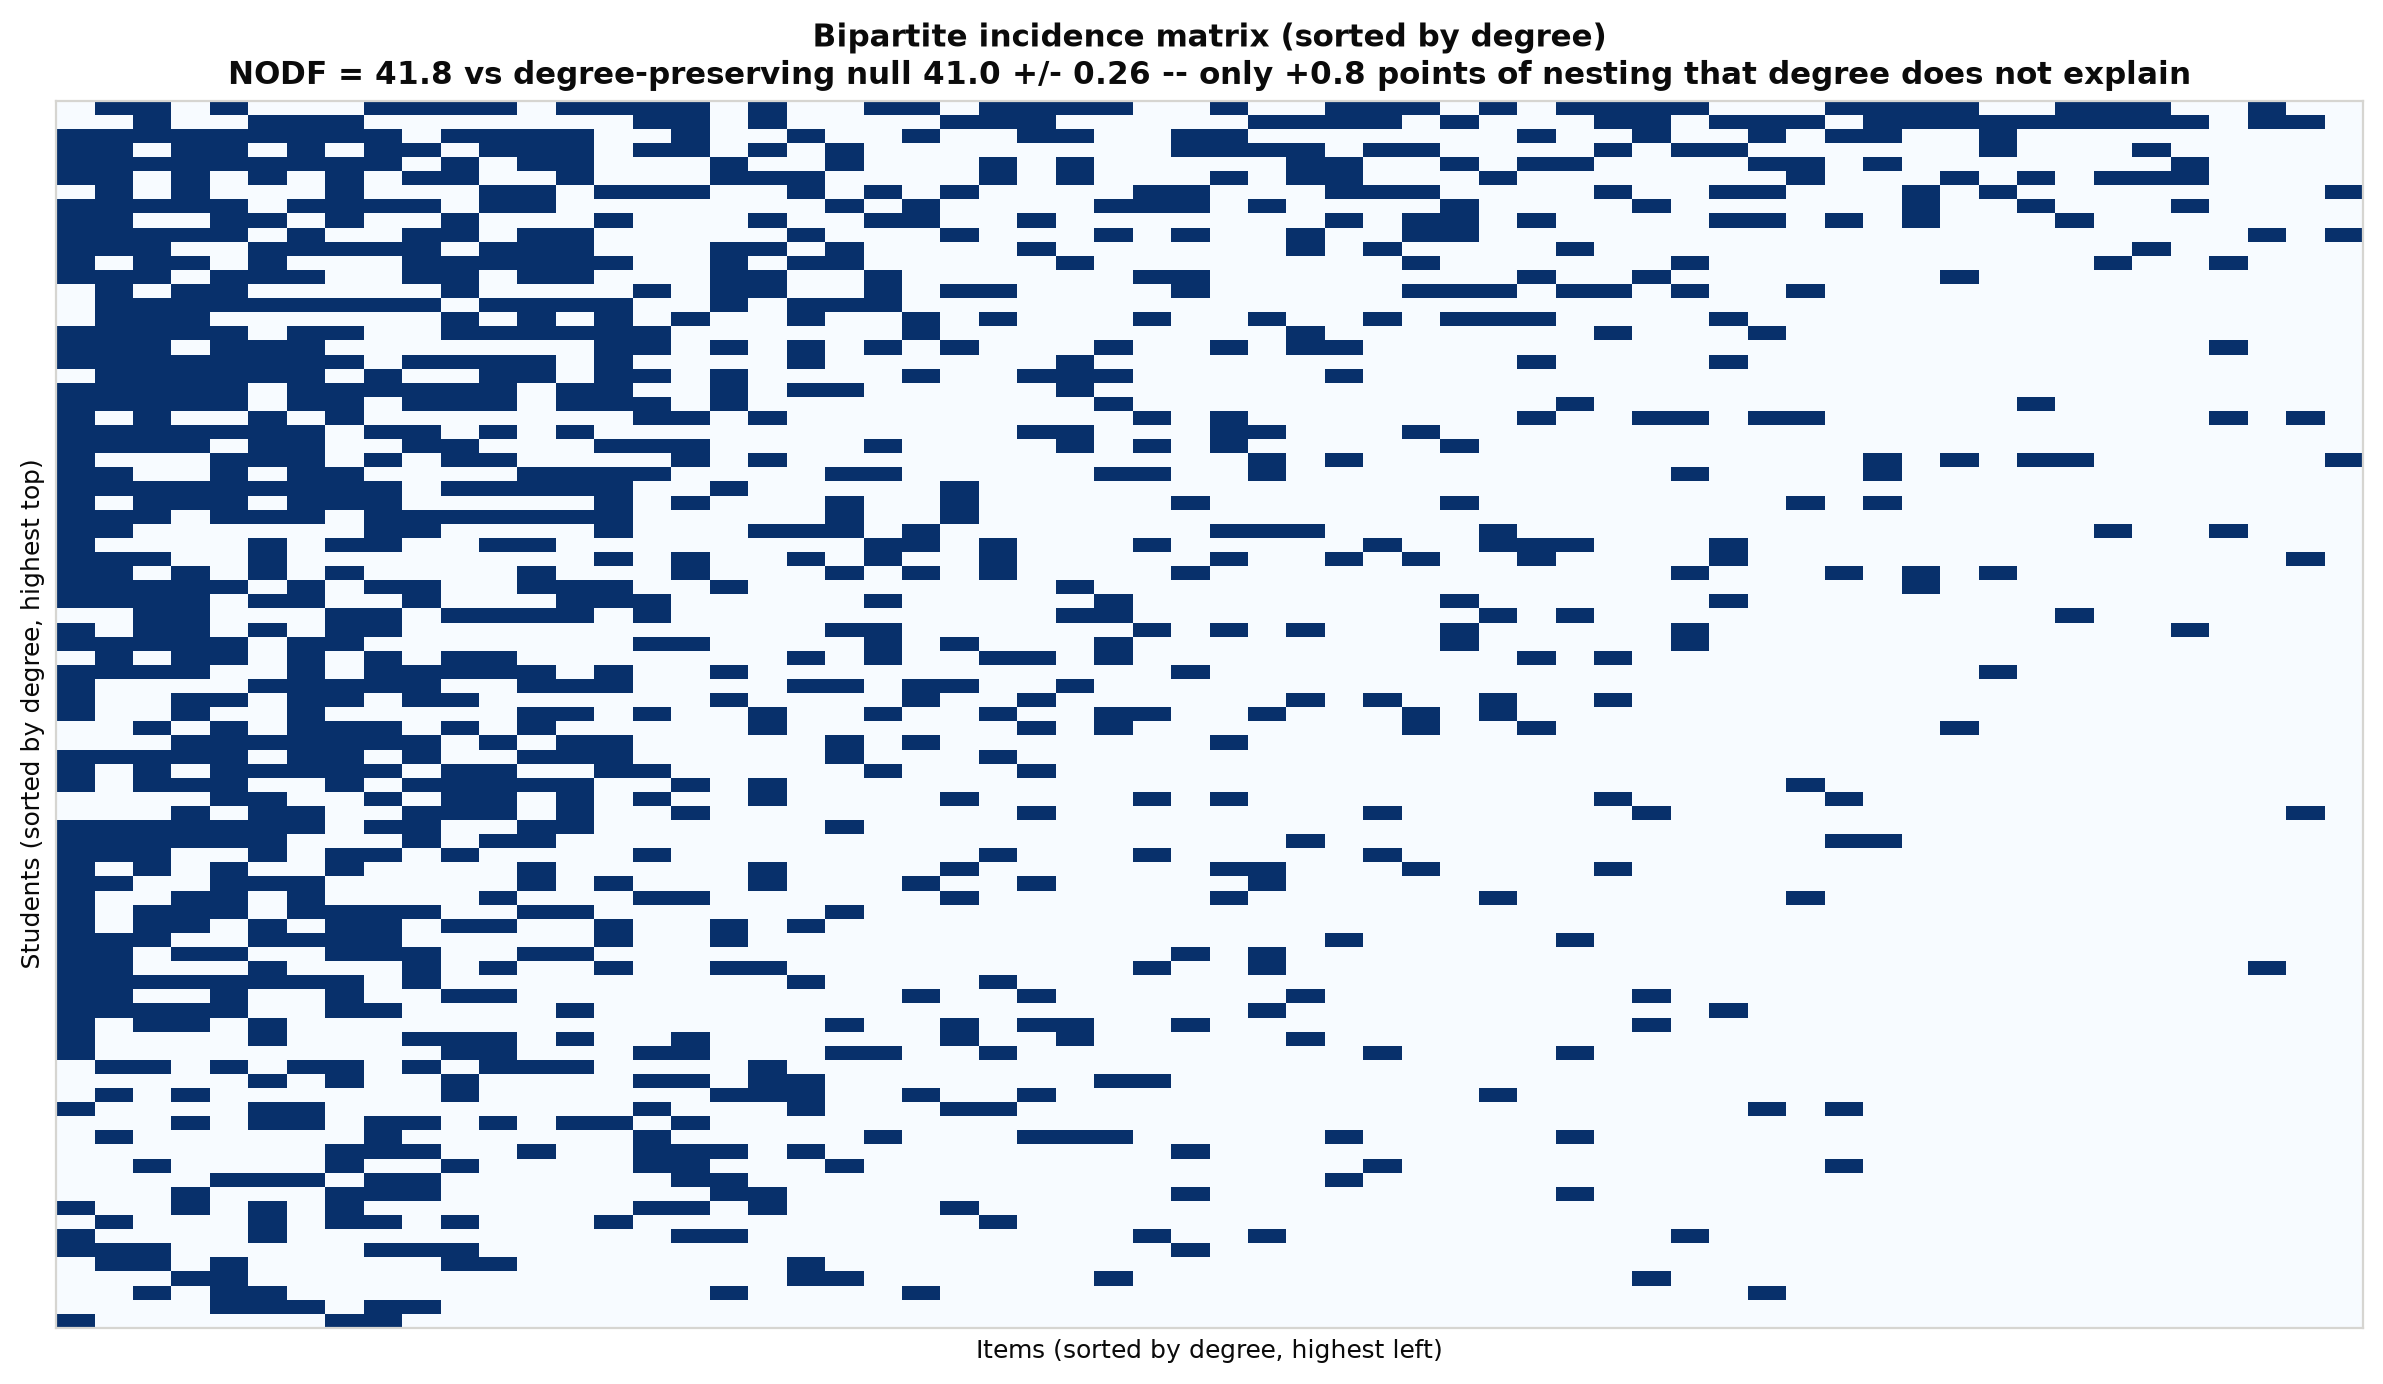
\includegraphics[width=0.62\textwidth]{../member_c_bipartite_net/figures/fig03_nestedness_matrix.png}
\caption{The bipartite incidence matrix, students by statements, sorted by degree. The
nested triangular shape is real but is almost entirely what the degree sequence alone
produces: only $+0.8$ NODF points of $100$ survive a null that fixes both degree
sequences.}
\end{figure}

\subsection{Running processes on these networks}

Structural measurement and dynamical behaviour do not always agree, and in this project
the dynamics repeatedly revealed things the static metrics concealed.

\textbf{A random walk on the deviation network is pure degree.} A walker alternating
student $\to$ item $\to$ student can only travel between students via an issue they both
deviate on, so mean first-passage time is an issue-mediated distance. Computed exactly
from the fundamental matrix with the true stationary distribution
$\pi_j \propto \mathrm{strength}_j$, MFPT spans $39.8$ to $1063.5$ steps --- a 27-fold
range that looks like rich structure. It is not. MFPT correlates with a student's
deviation degree at Spearman $\rho = -0.971$, and dividing node strength out leaves a
relative MFPT range of just $1.005$--$1.118$, hugging the degree-only expectation of
1.0. The deviation network is dynamically indistinguishable from a configuration model:
once you know how often a student deviates, you know essentially everything about how the
dynamics reach them. This is the same verdict the modularity and nestedness nulls
returned, arrived at by a third independent route.

\begin{figure}[h]
\centering
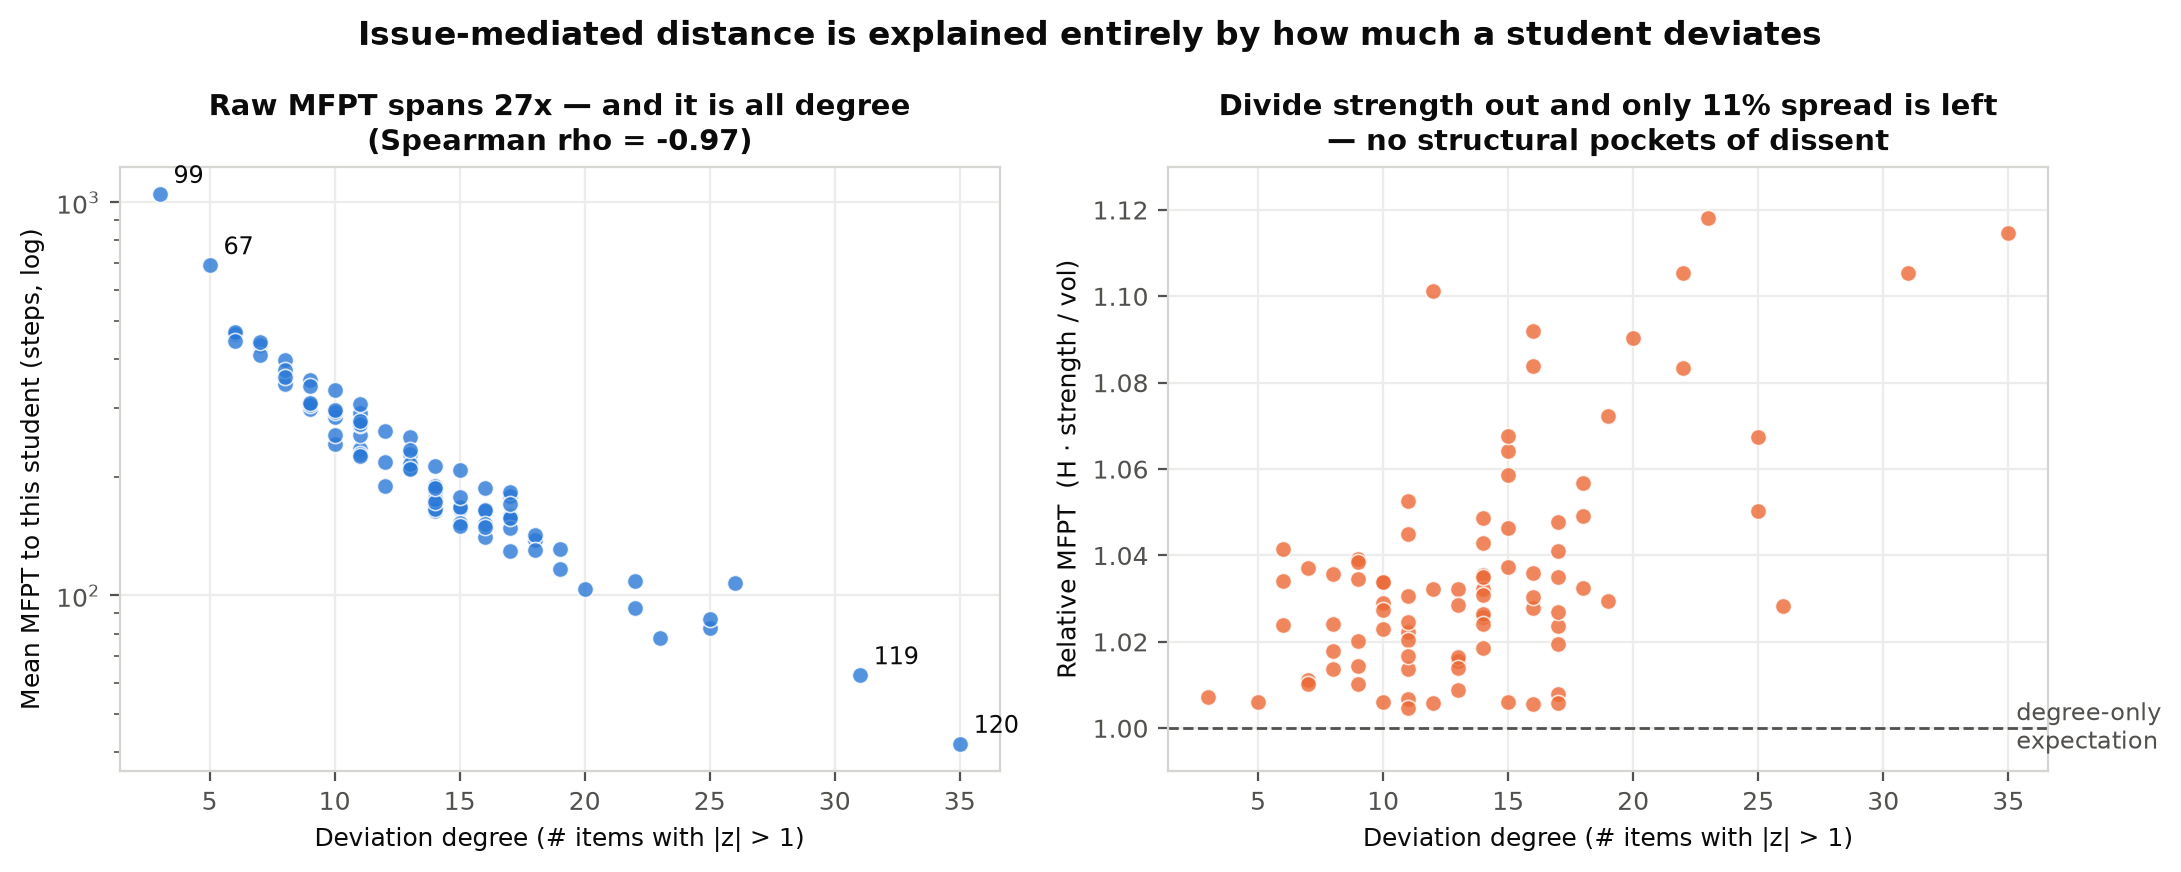
\includegraphics[width=0.92\textwidth]{../member_c_bipartite_net/figures/fig04_mfpt_structure.png}
\caption{Mean first-passage time on the bipartite deviation network. \textit{Left:} raw
MFPT spans 27-fold, but tracks deviation degree at $\rho = -0.971$. \textit{Right:}
dividing out node strength leaves only 11\% residual spread. There are no structural
pockets of dissent, no bottlenecks and no gatekeepers.}
\end{figure}

\textbf{Seeding the best-connected students backfires.} We ran SI spreading from three
seeds, 30 trials per condition, comparing seeds chosen by eigenvector centrality against
random seeds. On the dense threshold graph the choice is irrelevant: both reach
essentially the whole class. On the sparser mutual-$k$NN graph, centrality seeding is
actively worse, reaching $0.244 \pm 0.266$ of the class by $t=30$ against
$0.487 \pm 0.401$ for random seeds (mean $\pm$ SD over 30 trials; Welch
$t = 2.76$, $p = 0.008$). The spread deserves as much attention as the gap: on a graph
this sparse an outbreak either catches or dies, so the standard deviation is as large as
the mean and individual trials range from near-zero to near-complete coverage. The
difference in means is nonetheless reliable.

The mechanism is seed redundancy. Eigenvector centrality by construction rewards sitting
in the same dense core, so the three highest-scoring students are mutually adjacent ---
mean pairwise seed distance 1.00 hops, against 3.33 for random seeds on the same graph.
The three ``best'' seeds largely duplicate one another's reach. On a dense graph where
everyone is two hops from everyone, that redundancy costs nothing and the effect is
invisible; sparsify the same data and it becomes dominant. The textbook instinct to seed
the hubs fails here, and fails for a reason that only appears at low density.

\begin{figure}[h]
\centering
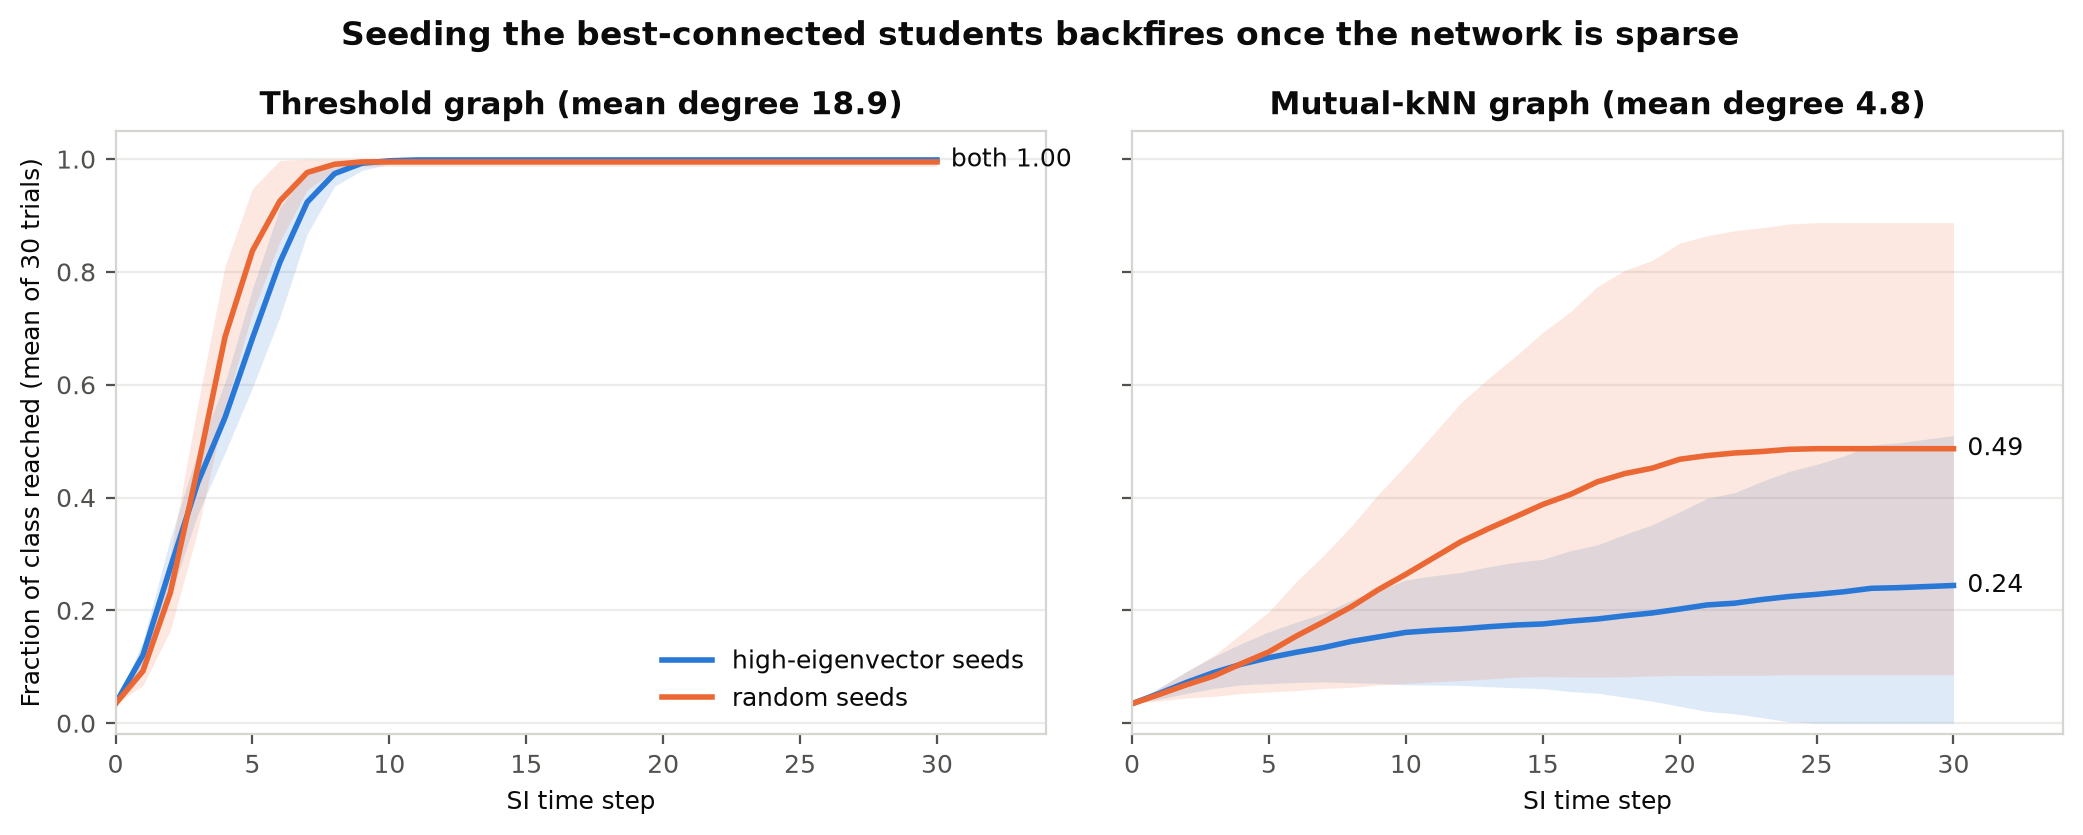
\includegraphics[width=0.92\textwidth]{../member_a_agreement_net/figures/fig08_si_seeding_density.png}
\caption{SI spreading from three seeds, 30 trials per condition, shading $\pm 1$ SD.
\textit{Left:} on the dense threshold graph the seeding strategy makes no difference.
\textit{Right:} on the sparse mutual-$k$NN graph random seeding reaches roughly twice as
many students on average, though the bands overlap heavily --- outcomes on a sparse graph
are close to all-or-nothing.}
\end{figure}

We also ran Deffuant--Weisbuch bounded-confidence dynamics on the agreement network and
Altafini signed consensus on the statement network. Both behaved exactly as their theory
predicts --- a fragmentation-to-consensus transition over $\varepsilon \approx 0.30$--$0.55$,
and slow monotone decay from $1.21$ to $0.08$, the expected signature of a nearly balanced
network. Neither distinguishes this class from any other, so we note them only in passing.

\section{Results and discussion}

\subsection{Two unrelated constructions rank the same statements the same way}

Member A measures, for each statement, the gap in mean $z$-score between the two student
blocs --- how sharply that statement separates the class. Member B measures, for each
statement, how far a perturbation propagates through the signed correlation network --- its
dynamical leverage. These quantities come from different graphs with different node sets
and different mathematics, and share nothing beyond the data contract. Across the 58
statements both can score, they agree at Spearman $\rho = +0.784$
($p = 3.5 \times 10^{-13}$; Pearson $r = +0.617$).

Aggregated by block they produce the identical ordering, \textbf{V $>$ S $>$ E $>$ T}:

\begin{table}[h]
\centering
\small
\begin{tabular}{@{}lccc@{}}
\toprule
\textbf{Block} & \textbf{A: mean $|z$-gap$|$} & \textbf{B: mean leverage} & \textbf{C: mean deviation degree} \\
\midrule
Environment (V) & 0.986 & $0.957 \pm 0.014$ & 14.13 \\
Society/Ethics (S) & 0.835 & $0.933 \pm 0.054$ & 19.33 \\
Education (E) & 0.536 & $0.762 \pm 0.235$ & 23.13 \\
Technology (T) & 0.434 & $0.714 \pm 0.249$ & 23.40 \\
\bottomrule
\end{tabular}
\end{table}

Beyond the means, the spread is striking. Environment's leverage has a standard deviation
of $0.014$ --- all fifteen V statements fall between $0.914$ and $0.967$. Technology's is
eighteen times larger at $0.249$, ranging from $0.233$ to $0.953$. Environment behaves as
one tightly coupled bloc in the opinion graph; Technology is a loose collection of
statements that happen to share a label. This is consistent with B's finding that the
class's own communities cut across the survey's topic blocks, and with T08 and T09
correlating with nothing at all.

\subsection{Influence and deviation run in opposite directions}

The third column of that table runs backwards, and deliberately so. Member C's deviation
degree --- how many students answered a statement more than one SD from the mean ---
anti-correlates with both other measures: $\rho = -0.390$ ($p = 0.002$) against B's
leverage, and $\rho = -0.349$ ($p = 0.006$) against A's bloc gap.

The statements that carry the most influence and most sharply divide the class are
precisely the statements individuals deviate from least. Environment is where the class is
most tightly coupled and most consensual, so V statements sort students into camps by
\textit{how strongly} they agree while attracting almost no individual dissent.
Technology and Education are where individuals actually break ranks.

Two senses of ``controversial'' turn out to be near-opposites, and the concrete case makes
it plain. B identifies E03 as the disagreement axis, carrying eight of eleven negative
edges. C identifies T13 as the biggest flashpoint, with 60 of 87 students deviating. Both
are right, because they measure different phenomena: E03 produces \textit{patterned
anti-correlation}, splitting the class into opposed sides, whereas T13 produces
\textit{raw spread}, making everyone answer differently from everyone else in no
particular pattern. Only having two networks makes the distinction visible.

\begin{figure}[h]
\centering
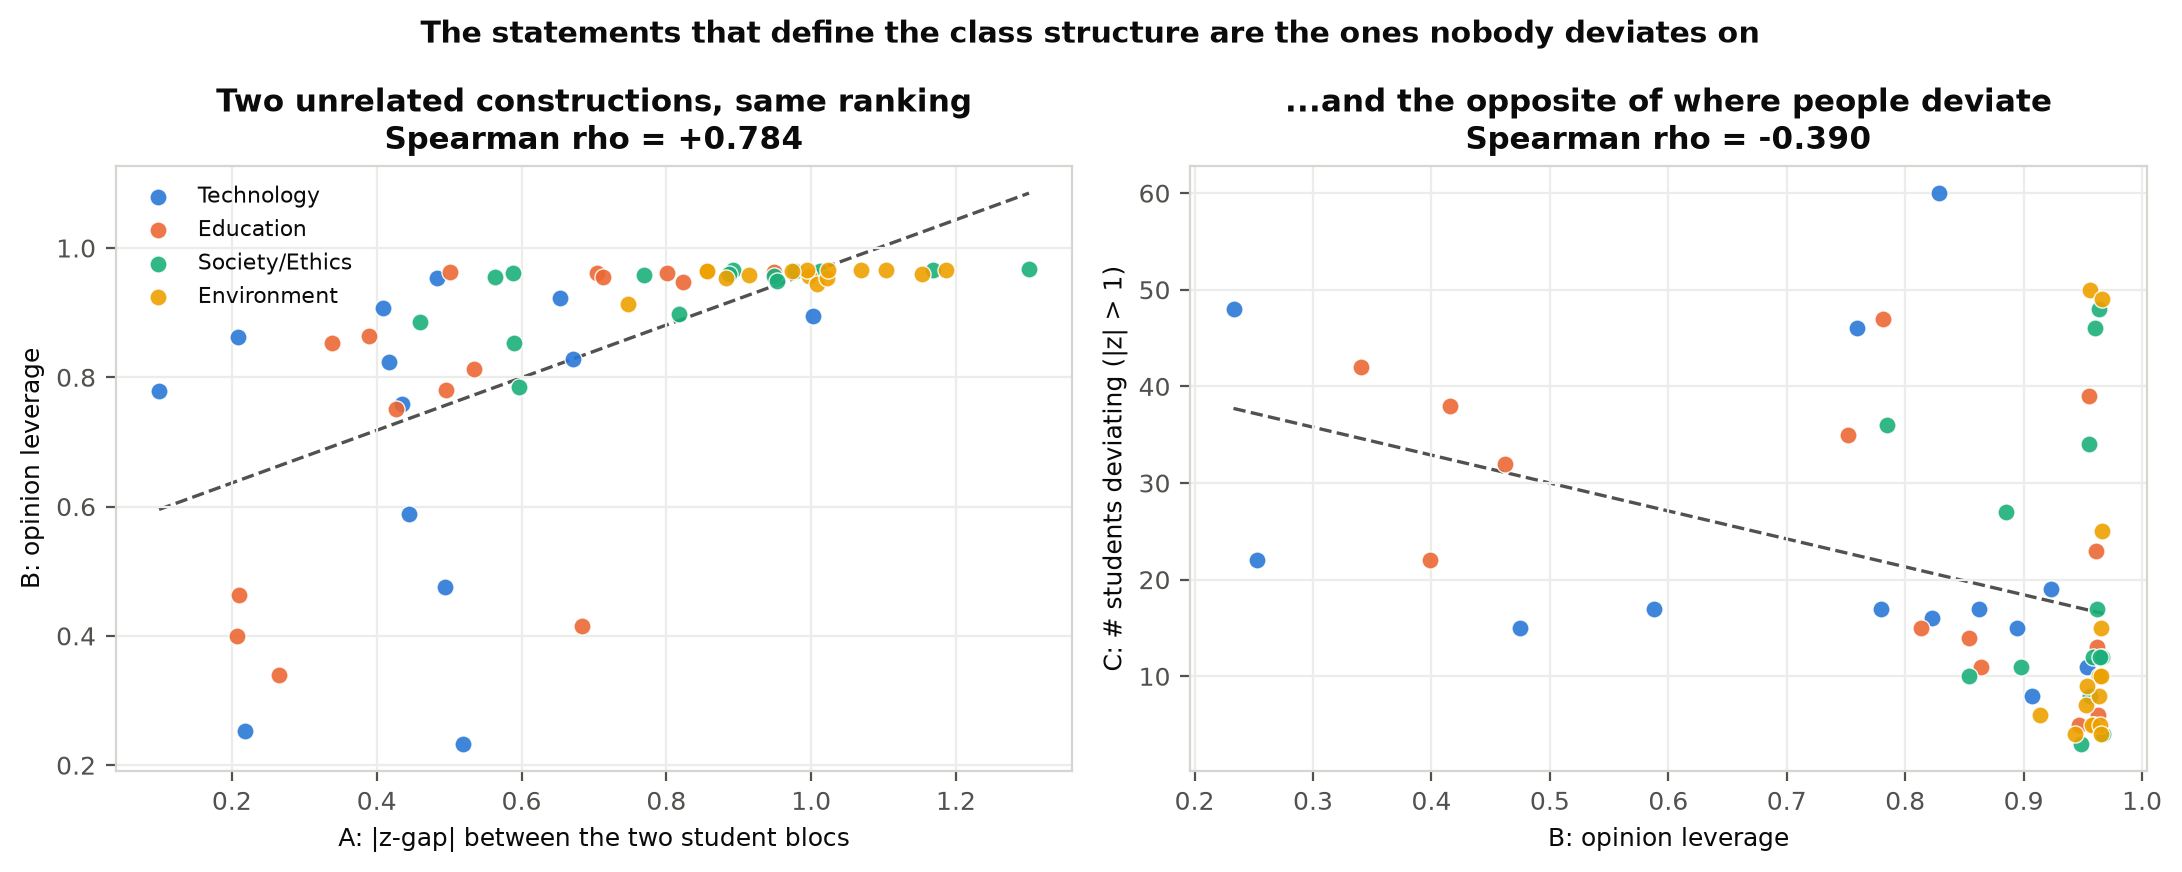
\includegraphics[width=0.92\textwidth]{../cross_analysis/figures/fig01_item_level_crosscheck.png}
\caption{\textit{Left:} two independent constructions rank the same 58 statements almost
identically. \textit{Right:} both run opposite to how much individual students deviate on
a statement. The saturation of leverage near $0.96$ means the positive relationship is
carried largely by the low-leverage tail, which is worth reading with some caution.}
\end{figure}

\subsection{What the three networks say together}

The single clearest result of this project is the asymmetry between agreement and
dissent. On the same 87 students, agreement structure sits $35.5$ standard deviations
above its null while co-dissent structure sits $6.1$ below its own. Three independent
measurements on network C --- modularity, nestedness and mean first-passage time --- all
return the same verdict: once you know how often a student deviates, you know essentially
everything about where they sit. Dissent in this class has volume but no shape.

That the two are genuinely different measurements, rather than two views of one
structure, is confirmed directly. Correlating A's pairwise agreement similarity against
C's symmetrised issue-mediated distance across 3741 student pairs gives
$r = +0.036$ ($\rho = +0.026$) --- explaining 0.1\% of variance. The Pearson $p$-value
clears $0.05$ only because 3741 pairs make trivial effects detectable, and we report this
as the null result it is. Knowing that two students think alike tells you essentially
nothing about whether they break from the class on the same questions.

Taken together, a coherent picture of this cohort emerges. It is a class that agrees
about most things and agrees \textit{consistently} --- clustering at 2.3 times the random
baseline, zero frustrated triangles out of 1298. Its real internal division is not
topical but temperamental, separating those who hold environmental and social positions
fervently from those who hold the same positions mildly. Its disagreements, where they
exist, are concentrated on a single coherent pedagogical axis rather than spread across
the survey. And its individual dissent is genuinely idiosyncratic: students depart from
consensus at very different rates, but which issues they depart on appears to be
personal rather than factional.

\subsection{Limitations}

The cohort is a single class of 87 respondents, so nothing here generalises beyond it.
The ceiling effect, while handled, still constrains what can be claimed: after
$z$-scoring we analyse residuals around a near-universal agreement, and the bloc we call
``moderate'' still agrees with most statements. Every network required a threshold, and
while coarse structure proved robust to all of them, specific edges did not --- A's two
edge rules share only a quarter of their edges. Claims about individual edges or students
should be read with that in mind; claims about blocs, blocks and null comparisons survive
the sweeps. Finally, leverage saturates near $0.96$, so the $\rho = +0.784$ agreement in
Figure 8 is carried disproportionately by the lower tail.

\section{Individual contribution}

Grading is individual, so each member owns one network end to end: its \texttt{src/}
modules, notebook, figures, tables, GEXF exports and \texttt{FINDINGS.md}. No member's
code imports another's.

\begin{table}[h]
\centering
\footnotesize
\begin{tabular}{@{}lp{12.9cm}@{}}
\toprule
\textbf{Member} & \textbf{Contribution} \\
\midrule
\textbf{Vishal} &
\texttt{member\_a\_agreement\_net/} --- the agreement network over 87 students. Edge-rule
design and the threshold/$k$NN/disparity comparison; percolation sweep; degree, clustering
and path structure; Louvain communities against configuration-model and
Erd\H{o}s--R\'enyi nulls; the community profiling that established the split is one of
intensity; centrality analysis separating hubs from bridges; and both dynamical processes
here, including the SI seeding experiment of Section 3.4. \\
\addlinespace
\textbf{Harith} &
\texttt{member\_b\_statement\_net/} --- the signed statement network over 60 statements.
Permutation-null edge construction with FDR control and the fixed-threshold sensitivity
comparison; degree and strength distributions; Louvain communities and the NMI comparison
against the survey's own T/E/S/V design; hub and isolate identification; the balance
analysis (triad census, frustration index, sign-shuffled null) and the E03 axis; Altafini
consensus dynamics and the leverage ranking used in Section 4.1. \\
\addlinespace
\textbf{Navneet} &
\texttt{member\_c\_bipartite\_net/} --- the bipartite student--statement deviation network.
Deviation-based construction and cutoff sensitivity; degree distributions on both sides
and flashpoint identification; NODF nestedness with its curveball degree-preserving null;
one-mode projections with the modularity null establishing that co-dissent falls below
chance; exact mean-first-passage-time analysis via the fundamental matrix, the
relative-MFPT correction, and the flashpoint-removal robustness experiment. \\
\addlinespace
\textbf{Joint} &
\texttt{common/} (the data contract and shared palette), agreed before any member wrote
analysis code; \texttt{cross\_analysis/} (Sections 4.1--4.2); and this report. The
conventions that make Section 4 possible --- shared cleaning, a null model for every
structural claim, sensitivity checks for every threshold, byte-identical re-runs --- were
agreed jointly in \texttt{development\_guidelines.md}. \\
\bottomrule
\end{tabular}
\end{table}

\end{document}
